\documentclass[11pt]{article}

\usepackage{fullpage}
\usepackage[numbers]{natbib}
\usepackage{amssymb}
\usepackage{amsmath}
\usepackage{bm}
\usepackage{bbm}
\usepackage{graphicx}
\usepackage{color}
\usepackage{hyperref}

\DeclareMathOperator{\erf}{erf}
\DeclareMathOperator{\lngamma}{\ln\!\Gamma}
\DeclareMathOperator{\Tr}{Tr}

% NOTE
% one sentence per line for nice git diffs
% WD: I'm a fan of initialed source comments like this


% WD: it's kinda silly to focus on unphased genomes then run on 1KG
\title{Population genetic reconstruction of mutation spectrum evolution from unphased genomes}

\author{
W.S. DeWitt$^{1,4}$, K. Decker Harris$^{2,3}$, and K. Harris$^{1,4}$\\
{\small
$^1$Department of Genome Sciences,
$^2$Paul G.\ Allen School of Computer Science \& Engineering,}\\
{\small and $^3$Department of Biology, University of Washington, Seattle, WA}\\
{\small $^4$Computational Biology Program, Fred Hutchinson Cancer Research Center, Seattle, WA}
% \small{$^\ast$ Equal contribution}
}

\begin{document}

\maketitle

\begin{abstract}

Models in evolutionary genetics typically assume that mutation rate is constant over time and between populations and closely related species.
However, recent work casts doubt on this assumption in human and ape populations, and reveals that mutation is a complex and dynamic process.
Whether arising from variation in replication fidelity, life history, or environmental exposures, mutation rate evolution can be accompanied by changes to the \emph{mutation spectrum}: the mutation rate in different local nucleotide contexts.
We extend theoretical tools based on Kingman's coalescent to accommodate a richly parameterized mutation process, varying in time and in spectrum.
% WD: revise below when we settle on what results will be in the paper
We infer human mutation spectrum histories from patterns of modern genomic diversity, allowing us to reconstruct trajectories of mutation spectrum divergence between populations, track a transient mutation spectrum perturbation through multiple populations, and characterize how mutation spectrum histories are structured by local nucleotide context.
Mutation rate and effective population size together determine the strength of genetic drift shaping genomic variation.
We introduce fast nonparametric joint inference of mutation spectrum history and demographic history from unphased genomes.

\end{abstract}


\section*{Introduction}\label{sec:intro}

% WD: should this be less humany?
Population genetics has proved to be a powerful lens on human history\cite{Harris2017-cd}, revealing a complex past of migration\cite{?}, replacement\cite{?}, and admixture among human groups and extinct homonids\cite{?}, and dramatic population size changes during and after range expansions\cite{?}.
Germline mutation events in the history of a population give rise to variant alleles, and demographic histories are recorded in patterns of segregation within and between current-day populations.
Genetic drift is shared when populations mix, and it is private during periods of isolation.
The strength of drift is universally influenced by the population size history, thus population genetic methods for demographic inference---expressed in the framework of Kimura's diffusion or Kingman's coalescent---attempt to recover the effective population size history $N(t)$.

Mutation drives the evolution of populations and species, and mutation rate evolution has a storied history in the theoretical population genetics literature.
Haldane developed equilibrium theory for alleles in mutation-selection balance, and used this to provided the first principled estimate of the human mutation rate by studying hemophilia incidence\cite{Haldane2004-ov, Nachman2004-gh}.
Kimura  \cite{Kimura1967-ku}

Storied history of theoretical treatments:
- Kimura: \cite{Kimura1967-ku}
- drift barrier hyp of \cite{Lynch2016-ff}

The process of germline mutation is the writing mechanism that records signatures of demographic events in genomes, so its influence on modern genome variation is similar in importance to the demographic histories themselves.
Demographic inference methods can model complex population splits, migration, and admixture, in addition to modeling $N(t)$ as a piecewise constant (or exponential) function of time into the past.
Mutation, however, receives a relatively impoverished treatment: usually a single mutation rate parameter $\mu$ is understood to apply at all loci in all individuals at all times, and may be regarded as a nuisance parameter needed for time calibration of models whose natural dimensionless time is measured in generations.

Growing evidence indicates that germline mutation is a dynamic process on both interspecific and population time scales, and a complex function of polymorphic replication machinery, life history, mutagenic exposures, and genomic content.
Indeed, mutation rates among great apes have declined along the lineage leading to humans---a phenomenon termed the \emph{homonoid slowdown}\cite{Goodman1985-xc, Scally2012-rb}---, showing that mutation rate evolution between species distorts phylogenetic time calibration.
Children of older parents receive more germline mutations, especially so for older fathers, and this is thought to arise from replicative errors in spermatogenesis.
This \emph{parental age effect} \cite{} indicates that life history changes can influence the population mutation process.
% need an example of mutagenic/spontaneous germline mutation


\begin{enumerate}
\item genomic regions (agarwal, and other Molly)
\item \texttt{C>T} at methylated CpGs due to deamination \cite{?}.
\item gbGC. We might want to talk about isochores here, but I've yet to find a coherent definition.
\item mutation spectra and pulse \cite{Harris2015-wi, Harris2017-fw}
\item Jed on context and regions \cite{Carlson2018-rc}
\item for some of these, it is unknown if driven by replicative Vs spontaneous mutation \cite{Gao2016-qp}, and that baboon paper touches on this (Molly)
\end{enumerate}

emerging picture of mutation rate accented by spectra

rare variant spectra \cite{Mathieson2017-rc} (maybe discuss normalization issues with this paper)

1KG cell line artifact \cite{Anderson-Trocme2019-fy} (they also use strict mask)

% this has to come after we into triplet spectra
Although methods exist for inferring locus-wise mutation rates \cite{Bhaskar2015-bd, Nelson2012-fr}, these require very large study sizes, and do not accommodate evolution of the rate or spectrum of the mutational process per se.

New methods that approximate the ancestral recombination graphs...

We have to be very clear about how what we’re offering is different than what can be done with Relate \cite{Speidel2019-ox}.
\begin{enumerate}
\item We can deal with unphased genomes.
\item Our method allows the total mutation rate to be variable whereas Relate fixes it to a constant, and does posthoc counting.
\item I do not quite understand how they count mutations in a given epoch, since they are not mapped to specific times, only to branches.
Unless mu(t) is constant, uniform sampling on the branch is not consistent
\item How does pulse timing compare?
\end{enumerate}

deserving more rich descriptions in population genetic models






% background:
% review on demographic inference (diff and coal methods), or popgen theory in general (Kimura's diffusion or Kingman's coal), and how they all assume a constant mu

% review on germline rate var: https://journals.plos.org/plosbiology/article?id=10.1371/journal.pbio.2000744

% Single nucleotide variant (SNV) frequencies partitioned according to local nucleotide context vary among human ancestry groups and among great ape species, indicating variation and divergence of the mutation process.

% moving beyond descriptive comparisons based on standing variation, to put mutation on the same footing as demographic history: "in the light of evolution" Dobzhansky

% models

% there is a family of models, simple panmictic coal, complex diff, psmc

% The sample frequency spectrum (SFS)---the distribution of derived allele frequencies among sampled haplotypes---is a well-studied population genetic summary statistic that is sensitive to demographic history.

% gloom and doom perils about N(t), Meyers, Song, other Song, Gravel, etc., nonlinearity, nonconvexity, then contrast this with our discovery of a more tractable problem
% This has a truly excellent intro/summary of the issues with the SFS: https://www.sciencedirect.com/science/article/pii/S004058091730148X?via%3Dihub

% "Stairway plot" that Kern recommended, is sort non-parametric: X. Liu, Y.-X. Fu, Exploring population size changes using SNP frequency spectra. Nat. Genet. 47, 555–559 (2015).

% We extend a coalescent framework for demographic inference from the SFS to accommodate inference of mutation spectrum histories from the sample frequency spectrum resolved by $k$-mer nucleotide context ($k$-SFS).
% We formulate inference of mutation spectrum histories from the $k$-SFS as a linear inverse problem.

% as the first method like this, we implement in the simpler among models in the family, single population. Beginning of fruitful future work to bring model realism to popgen inf, via much more rich descriptions of the mutational process.

% sims with realistic demo hist and various spectrum hists, we can recover

% github



% TODO
% - ancient african substructure buzz, bantu VS san, admixture signal?
% - gbGC and isochores: https://www.annualreviews.org/doi/abs/10.1146/annurev-genom-082908-150001?casa_token=EImkIpqbayAAAAAA:Rxc8y0KLVRbZ6UfBTy3VxBRPdt3IZf7CAdVk57DfBUpvpSvuP4uHpDe9XHHCMHFBbYDxcZyFR8t0tA


\cite{Harris2017-fw} showed triplet SNV spectrum differences between human groups and between great apes, and used a coalescent simulation approach to fit the timing of a pulse of \texttt{T\underline{C}C>T\underline{T}C} mutations in Europeans.
We develop coalescent theory for the dependence of the expected $k$-SFS on both demographic history (effective population size as a function of time into the past) \emph{and} mutation spectrum history (mutation intensities as a function of time into the past for each mutation type).
This is similar in spirit to Kelley's simulation-based approach (which assumed the European demography of \cite{Tennessen2012-dq}), but is much faster, more flexibly parameterized.

Some references for nonidentifiability of demographic history from the SFS: \cite{Baharian2018-np, Bhaskar2014-fu, Terhorst2015-xt, Myers2008-jp}.
It might be good to consider identifiability of mutation intensity history from the SFS conditioned on demographic history.

% WD: todo: inverse problem intro, forward Vs inverse problems, and ill-posedness. Point out \eta is nonlinear, but \mu is linear

% WD: todo: the scope of this paper is \mu inference conditioned on \eta. There are plenty of fancy methods one can use to infer \eta

% Humblebrag: the word \emph{spectrum} is triply overloaded in this paper:
% \begin{enumerate}
% \item the traditional sample frequency \emph{spectrum}
% \item mutation \emph{spectrum} as in the nucleotide context of each mutation
% \item \emph{spectral} regularization for encouraging low rank solutions
% \end{enumerate}

\section*{Model}\label{sec:model}

The setting for our modeling is Kingman's coalescent \cite{Kingman1982-ge, Kingman1982-tf, Kingman1982-ys, Kingman2000-jr}, with all the usual niceties: neutrality, infinite sites, linkage equilibrium, and panmixia.
In Appendix \ref{sec:appendix} we detail our retracing of the derivation by \cite{Griffiths1998-qf} of the frequency distribution of a derived allele conditioned on the demographic history, while generalizing to a time inhomogeneous mutation process.
We make use of the results of \cite{Polanski2003-kg} and \cite{Polanski2003-ll} to facilitate computation, and build on the notation of \cite{Rosen2018-bb} for a finite-dimensional approximation of our demographic and mutation intensity histories.
Complete derivation of formulae are found in the Appendix.

Given $n$ sampled haplotypes and a demographic history $\eta(t)$ (with time measured retrospectively from the present), we show in Appendix \ref{sec:appendix:xi} that the expected SFS $\boldsymbol \xi = (\xi_1, \xi_2,\dots, \xi_{n-1})$ is a linear transform of the mutation intensity history $\mu(t)$:
\begin{equation}
  \label{eqn:transform}
\boldsymbol \xi = \mathcal{L}_{n,\eta(t)}\mu(t),
\end{equation}
where $\mathcal{L}_{n,\eta(t)}$ is a finite-rank linear operator that maps infinite-dimensional mutation intensity histories to $(n-1)$-dimensional SFS vectors.
It is dependent on $n$ and $\eta$, which we take to be fixed.

% Need to talk about this fig \ref{fig:model}.

\begin{figure}
\centering
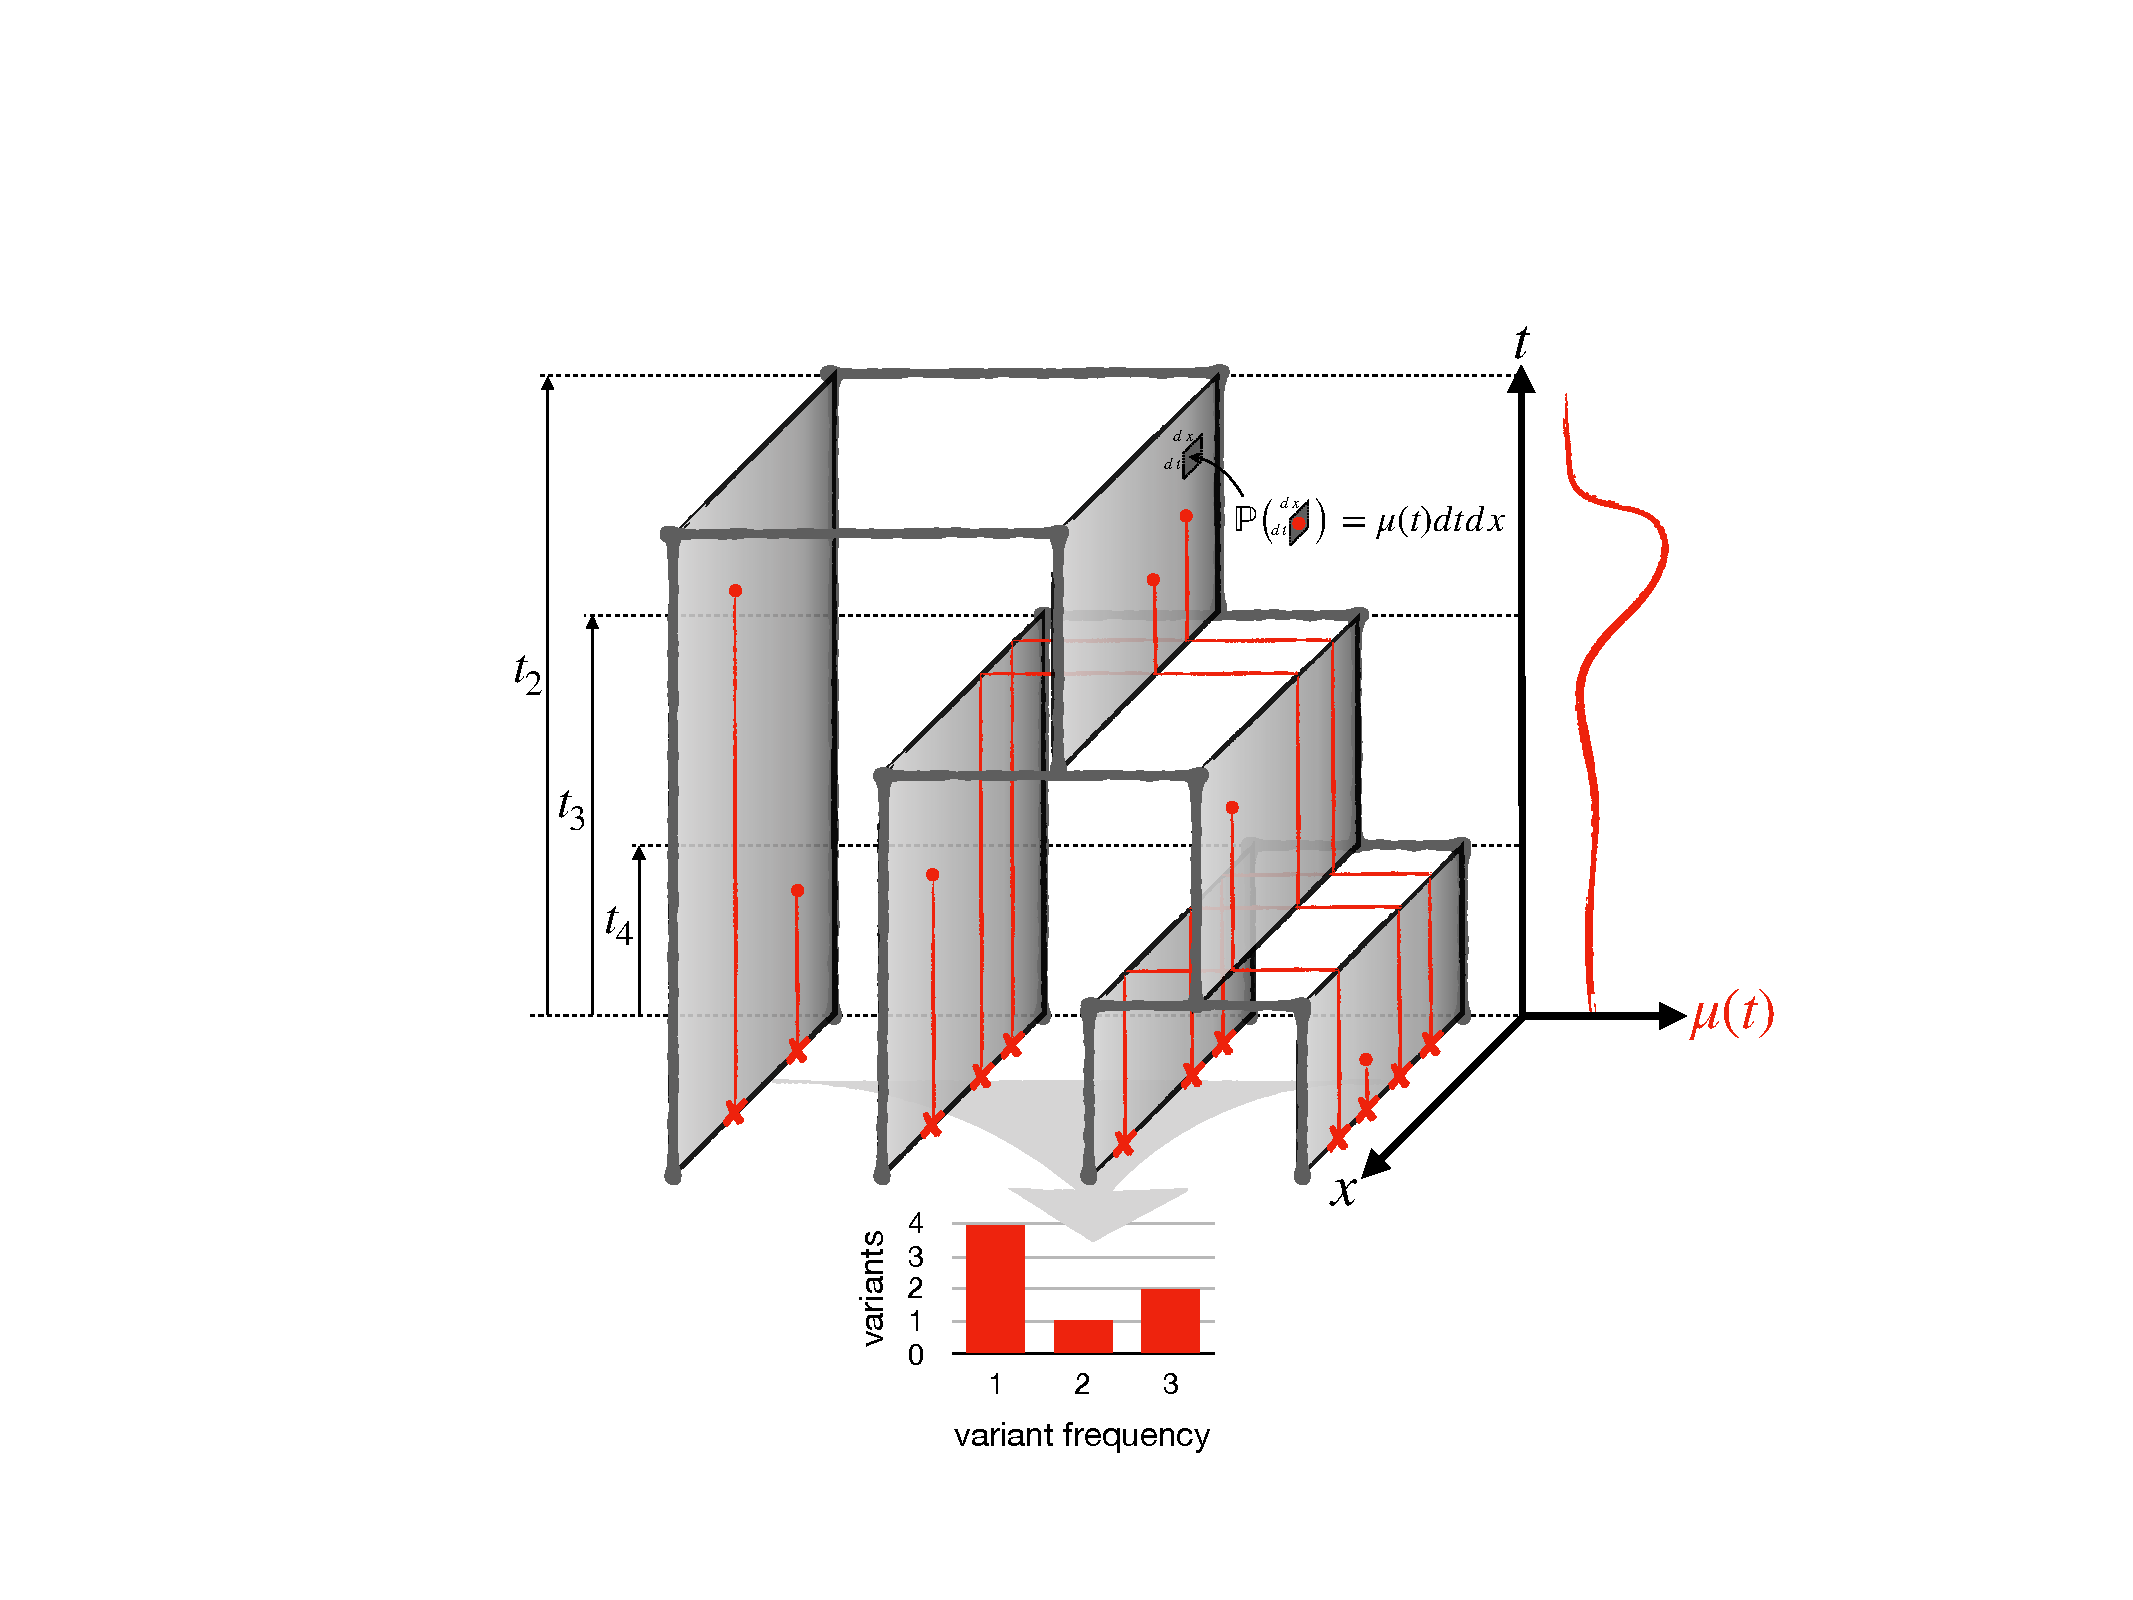
\includegraphics[width=\textwidth]{figures/model}
\caption{Schematic of the marked Poisson process model with $n=4$.
We condition on coalescent times $T_4=t_4,T_3=t_3,T_2=t_2$ and consider mutation intensity function $\mu(t)$.
Red dots indicate mutation events placed by time $t$, genomic position $x$, and coalescent line (which are depicted as extruded in the genomic coordinate axis, grey sheets).
The probability that a differential element $dxdt$ on a given sheet contains a mutation is proportional to the instantaneous mutation intensity $\mu(t)$.
}
\label{fig:model}
\end{figure}

In previous work \cite{Kelley, cancer, etc}, mutation spectra have been parameterized by grouping variants into mutation types according to local $k$-mer nucleotide context, and the number of variants called in each mutation type is taken as a proxy integrating an individual's ancestral mutational input in each type.
With $k$ odd and the variant registered in the central position there are $\kappa_k=2\times3\times4^{k-1}$ mutation types after collapsing by strand symmetry.
For example, there are $96$ triplet mutation types ($k=3$).
Here, we use the same $k$-mer mutation type parameterization to promote the $(n-1)$-element expected SFS vector $\xi$ to the $(n-1)\times\kappa_k$ expected $k$-SFS matrix $\Xi$.
Similarly, the mutation intensity history function $\mu(t)$ is promoted to the $\kappa_k$-element mutation spectrum history $\boldsymbol\mu(t)$, with each element giving the mutation intensity history function for one mutation type.
Equation \eqref{eqn:transform} becomes
\begin{equation}
  \label{eqn:transform_matrix}
\Xi = \mathcal{L}_{n,\eta(t)}\boldsymbol\mu^\intercal(t),
\end{equation}

For numerical implementation we consider finite-dimensional approximations of $\eta(t)$ and $\boldsymbol\mu(t)$ as piecewise constant functions of time on $m$ common epochs $[t_0, t_1), [t_1, t_2),\dots, [t_{m-1}, t_m)$ where $0=t_0 < t_1 < \dots < t_{m-1} < t_m=\infty$.
We take the epoch boundaries as fixed parameters, and in practice make them dense so as to approximate infinite-dimensional histories.
Let $\boldsymbol y = (y_1,\dots,y_m)$ denote the constant population size $\eta(t)$ during each epoch, and let the $m\times\kappa_k$ matrix $Z$ denote the constant mutation intensity during each epoch (rows) for each mutation type (columns).
In Appendix \ref{sec:appendix:pcsws} we show the linear transform \eqref{eqn:transform_matrix} reduces to the matrix equation
\begin{equation}
\label{eqn:transform_discrete}
\Xi = L_{n, \boldsymbol y} Z,
\end{equation}
where the $(n-1)\times m$ matrix $L_{n, \boldsymbol y}$ is fixed given a fixed demographic history $\boldsymbol y$.

In linkage equilibrium the log likelihood function of the mutation spectrum history $Z$ given an observed $k$-SFS matrix $X$ and demographic history $\boldsymbol y$ is given by the Poisson random field approximation \cite{?}
\[
\ell(Z; X, \boldsymbol y, n) = \Tr(X^\intercal\log(L_{n, \boldsymbol y} Z)) - \|L_{n, \boldsymbol y} Z\|_1,
\]
where $\log(\cdot)$ operates elementwise, and we've dropped a constant term wrt $Z$.

% WD: more inverse problem intro
The inverse problem \eqref{eqn:transform_discrete} is ill-posed in general,
so many very different histories can be equally consistent with the data
\cite{oscillation paper? Yun's other papers?}.
We deal with this problem using regularization, to enforce well-behaved histories.
Our cost function to minimize, a penalized log-likelihood, is
\begin{equation}
\label{eqn:penalized}
C(Z)
%\tilde\ell(\boldsymbol z)
= -\ell(Z) + R(Z) .
\end{equation}
The function $R(Z)$ incorporates our regularization.
In order to recover smooth histories,
we penalize the $L^p$ norms
of the time derivative of $\boldsymbol\mu(t)$
\[
\sum_{i=1}^{\kappa_k}\left\| \frac{d \mu_i(t)}{d t} \right\|_p^p
= \sum_{i=1}^{\kappa_k}\int_0^\infty\left|\frac{d\mu_i(t)}{dt}\right|^p dt,
\]
for $p=1,2$.
With piecewise constant histories as in \eqref{eqn:transform_discrete} this becomes
\[
\left\|\Delta Z \right\|_p^p.
\]
where $\Delta$ denotes the first difference matrix.
When $p = 1$, this is referred to as a fused LASSO or total variation (TV) penalty,
whereas $p=2$ is called a spline penalty.
We have implemented three different types of regularization.

The first option we call ``soft'' rank regularization, with
\begin{equation}
  \label{eq:regularization_soft}
  R_\mathrm{soft}(Z)
  =
  \frac{  \lambda_\mathrm{spline} }{2} \left\|\Delta Z\right\|_2^2
  +
  \lambda_\mathrm{rank} \| Z \|_*
  +
   \frac{\lambda_\mathrm{ridge}}{2}  \| Z \|_\mathrm{F}^2
   .
\end{equation}
The spline term controls the smoothness of solutions,
and the rank term allows us to recover low-rank solutions.
The rank penalty is the nuclear norm $\| Z \|_*$,
which is equivalent to the $\ell^1$-norm on the singular values.
If $Z = U S V^\intercal$ is the SVD of $Z$, with $S = \mathrm{diag}(\sigma)$ then $\| Z \|_* = \| \sigma \|_1$.
The parameters $\lambda_\mathrm{spline}$ and $\lambda_\mathrm{rank}$ control the overall strength
of smoothing and rank regularization.
The function $R_\mathrm{soft}$ is convex; therefore we have a convex optimization problem
in this scenario.

The second option is ``hard'' rank regularization, where
\begin{equation}
  \label{eq:regularization_soft}
  R_\mathrm{hard}(Z)
  =
  \frac{\lambda_\mathrm{spline}}{2} \left\|\Delta Z\right\|_2^2
  +
  \lambda_\mathrm{rank} \, \mathrm{rank}(Z)
  +
  \frac{\lambda_\mathrm{ridge}}{2} \| Z \|_\mathrm{F}^2
  .
\end{equation}
Here, the rank penalty is the actual rank of $Z$,
and note that $\mathrm{rank}(Z) = \| \sigma \|_0$.
In this case the problem is {\em not} convex.
However, we may still compute a proximal map for the non-differentiable rank term
and optimize with prox-gradients.

The third option allows more general smoothing but ignores all rank penalization:
\begin{equation}
  \label{eq:regularization_soft}
  R_\mathrm{indep}(Z)
  =
  \lambda_\mathrm{TV}
  \left\|\Delta Z\right\|_1
  +
  \frac{\lambda_\mathrm{spline}}{2} \left\|\Delta Z\right\|_2^2
  +
  \frac{\lambda_\mathrm{ridge}}{2} \| Z \|_\mathrm{F}^2
  .
\end{equation}
The TV terms control the smoothness of solutions,
and the rank term allows us to recover low-rank solutions.
The function $R_\mathrm{indep}$ is convex.
Note also that the columns of $Z$ are uncoupled,
so that we may solve this case as $\kappa_k$ different subproblems.


\section*{Results}\label{sec:results}

% Todo:
% \begin{itemize}
% \item repeat 1KG analysis like in \cite{Harris2017-fw}, see if we recapitulate Kelley's simulation-based pulse results
% \item cluster triplet time series to see if we pull in minor components.
% \end{itemize}

\begin{figure}
  \centering
  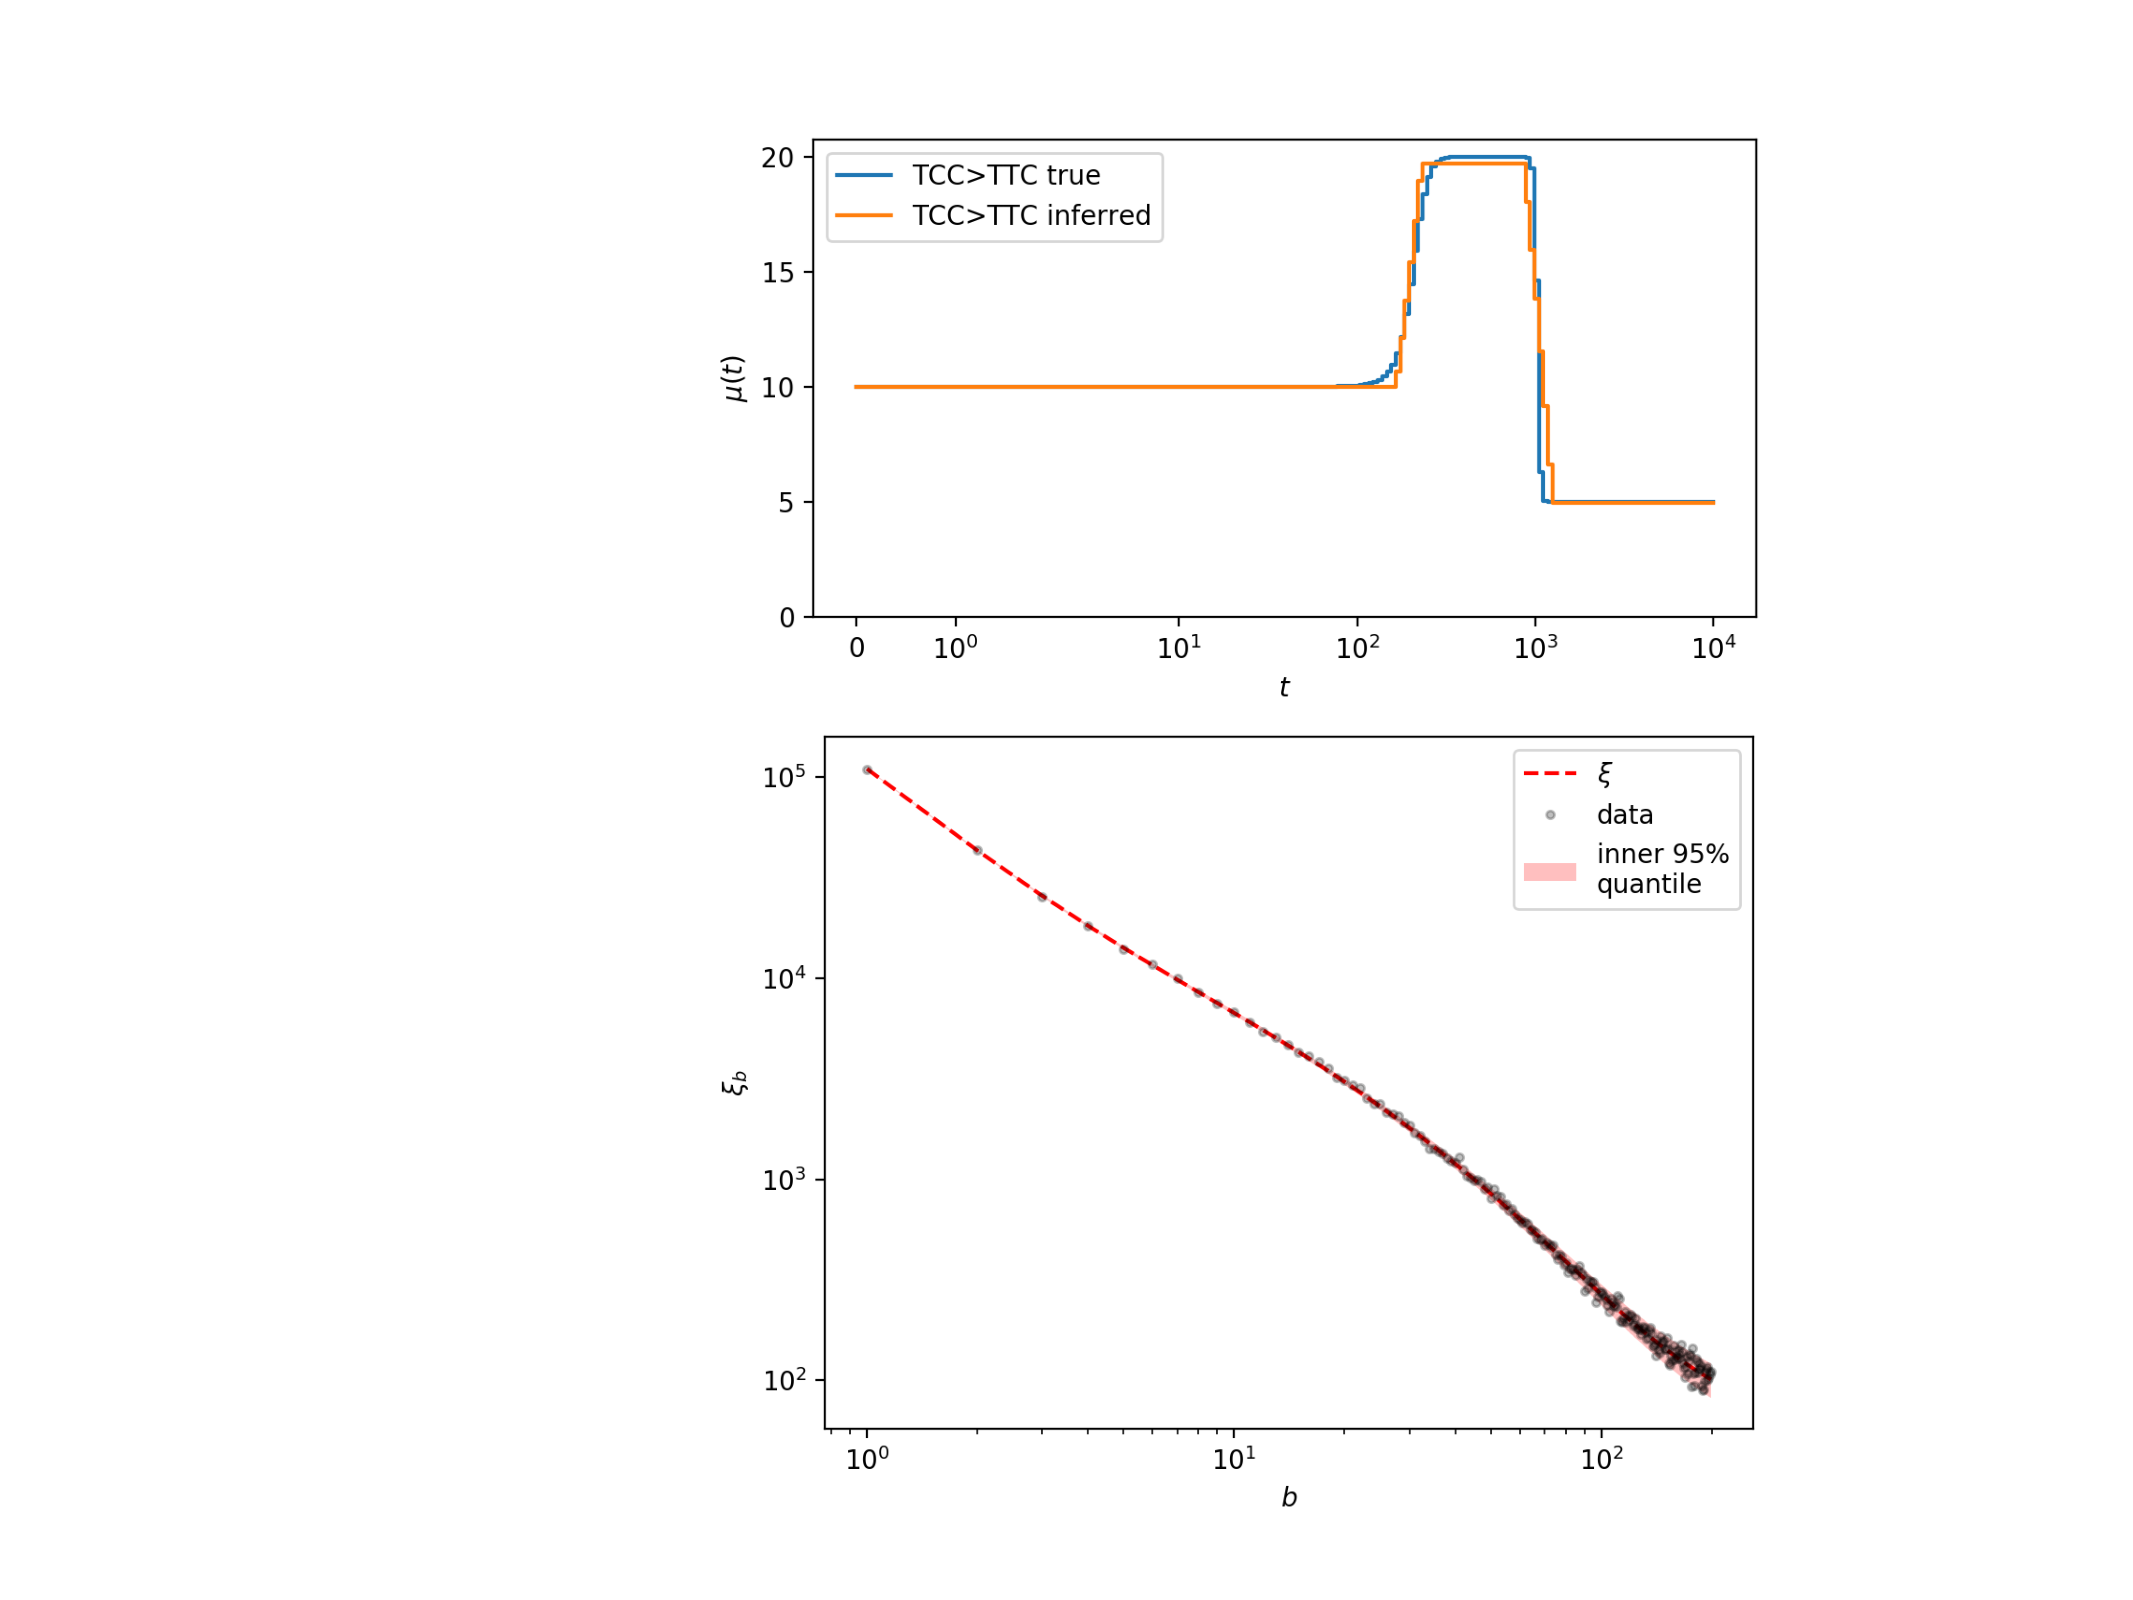
\includegraphics[width=.7\textwidth]{figures/fit_teaser}
  \caption{Simulating and inverting a pulse.}
  \label{}
\end{figure}

\subsection*{Tempora incognita: observability toward the coalescent horizon}\label{sec:model:loss}

Todo: SVD on $L_{n, \boldsymbol y}$

Intuitively, we know the SFS can't contain any information about the history beyond the TMRCA $T_2$, since mutations that occurred before then will not be segregating in the sample.
Thus, we will find it useful to penalize complexity in the history more heavily at times that are more probably ancestral to the TMRCA.

From \eqref{eqn:pi} and \eqref{eqn:r} in the Appendix \ref{sec:appendix}, the CDF of $T_2$ is
\begin{align}
F_2(t) &= 1 - \sum_{j=2}^n A_{2,j}r_2(t)\\
&= 1 - \sum_{j=2}^n A_{2,j}r_2(t)
\end{align}


\section*{Discussion}\label{sec:discussion}

Joint inference of $\eta$ and $\mu$.


\section*{Methods}\label{sec:methods}

\subsection*{Implementation and pipeline}\label{sec:methods:tool}

The \texttt{mushi} software package is available at \url{https://github.com/harrispopgen/mushi}.
% WD: cite whatever packages we use, e.g. jax, proxtv, msprime, stdpopsim, etc.

\section*{Acknowledgements}\label{sec:ack}

Erick Matsen, Peter Ralph, Andy Kern, Harris lab, Jeff Spence, Aleksandr Aravkin

\bibliographystyle{plainnat}
\bibliography{refs}


\appendix
\section{Appendix}\label{sec:appendix}

\subsection{The expected SFS given demographic and mutation intensity histories}\label{sec:appendix:xi}

Suppose $n$ haplotypes are sampled in the present, and let rvs $(T = T_2,\dots,T_n)$ denote the coalescent times measured retrospectively from the present (i.e. $T_n$ is the most recent coalescent time, and $T_2$ is the TMRCA of the sample).
As in \cite{Griffiths1998-qf} \S3, we consider a marked Poisson process in which every mutation is assigned a random label drawn iid from the uniform distribution on $(0,1)$.
This is tantamount to the infinite sites assumption, with the unit interval representing the genome, and the random variate labels representing mutant sites.
%WD Kam suggests replacing below with $\mu^* \ge \mu(t) \ge 0$, but I don't get why
Further suppose that mutation intensity is not constant, but a specified function of time $0\le \mu(t)<\infty$ (measured in mutations per genome per generation) applying equally to all lines in the coalescent tree at a given time $t$ (measured retrospectively from the present in units of Wright-Fisher generations).
A given line in the coalescent tree then acquires mutations on a genomic subinterval $(x,x+\delta x)$ at rate $\mu(t)\delta x$.
The following argument can be generalized to allow the labelling distribution to be nonuniform over the unit interval, but the same results follow.

Let rv $\mathcal{E}_{\delta x, b}$ denote the event that a mutation present in $b\in\{1, 2, \dots, n-1\}$ haplotypes in the sample occurred within a given genomic interval $(x,x+\delta x)$ (the probability of this event is independent of $x$, given the uniform labeling distribution).
Let $I_k$ denote the $k$th intercoalescent time interval, i.e.\ $I_n = (0, T_n),\ I_{n-1} = (T_n, T_{n-1}),\ \dots,\ I_2 = (T_3, T_2)$.
Let rv $\mathcal{E}_{\delta x, b, k}$ denote the event that the mutation $\mathcal{E}_{\delta x, b}$ occurred during $I_k$.
For small $\delta x$ and finite $\mu(t)$ we have
\begin{align*}
\mathbbm{P}(\mathcal{E}_{\delta x, b}\mid T) &= \sum_{k=2}^n \mathbbm{P}(\mathcal{E}_{\delta x, b, k}\mid T)\\
&= \sum_{k=2}^n p_{n,k}(b)\left(k\delta x\int_{t\in I_k}\mu(t)dt + O((\delta x)^2)\right),
\end{align*}
where
\begin{equation}
\label{eqn:p}
p_{n,k}(b) = \frac{\binom{n-b-1}{k-2}}{\binom{n-1}{k-1}}
\end{equation}
is the probability that a mutant that arose when there were $k$ ancestral lines of $n$ sampled haplotypes will be present in $b$ of them (see \cite{Griffiths1998-qf} eqn 1.9), and the quantity in parentheses is the probability that a mutation arose during the $k$th intercoalescent interval in a small genomic interval of size $\delta x$.
Marginalizing $T$ gives
\begin{align*}
\mathbbm{P}(\mathcal{E}_{\delta x, b}) &= \delta x\sum_{k=2}^n k p_{n,k}(b) \mathbbm{E}_T\left[\int_{t\in I_k}\mu(t)dt\right] + O((\delta x)^2).
\end{align*}
For small $\delta x$, each such interval contains zero or one mutations, so the expected number of mutations subtending $b$ haplotypes (i.e.\ the $b$th component of the SFS) is
\[
\xi_b = \int_0^1 \mathbbm{P}(\mathcal{E}_{dx, b})dx = \sum_{k=2}^n k p_{n,k}(b)\mathbbm{E}_T\left[\int_{t\in I_k}\mu(t)dt\right]\nonumber
\]
Using the explicit bounds of the intercoalescent intervals, $I_{k} = (T_{k+1}, T_k)$, gives
\begin{align}
\label{eqn:xi}
\xi_b &= \sum_{k=2}^n k p_{n,k}(b) \mathbbm{E}_{T_k}\left[\int_0^{T_k}\mu(t)dt\right] - \sum_{k=2}^{n-1} k p_{n,k}(b) \mathbbm{E}_{T_{k+1}}\left[\int_0^{T_{k+1}}\mu(t)dt\right]\nonumber\\
&= \sum_{k=2}^n k p_{n,k}(b) \mathbbm{E}_{T_k}\left[\int_0^{T_k}\mu(t)dt\right] - \sum_{k=3}^{n} (k-1) p_{n,k-1}(b) \mathbbm{E}_{T_{k}}\left[\int_0^{T_k}\mu(t)dt\right]\nonumber\\
&= \sum_{k=2}^n B_{b,k} \mathbbm{E}_{T_k}\left[\int_0^{T_k}\mu(t)dt\right],
\end{align}
where
\begin{equation}
\label{eqn:B}
B_{b,k}\equiv
\begin{cases}
k p_{n,k}(b),& k=2\\
k p_{n,k}(b) - (k-1) p_{n,k-1}(b),& k > 2
\end{cases}
\end{equation}

\cite{Polanski2003-kg} (eqns 5-8) give the marginal density for the coalescent time $T_k$ as
\begin{equation}
\label{eqn:pi}
\pi_k(t_k) = \sum_{j=k}^n A_{k,j} q_j(t_k)
\end{equation}
where
\begin{align*}
A_{k,j} &\equiv \frac{\prod_{l=k\ne j}^{n}\binom{l}{2}}{\prod_{l=k\ne j}^{n}\left[\binom{l}{2}-\binom{j}{2}\right]}, k\le j\le n,\\
A_{n,n} &\equiv 1,\\
q_j(t) &\equiv \frac{\binom{j}{2}}{\eta(t)}\exp\left[-\binom{j}{2}\int_0^t\frac{dx}{\eta(x)}\right],
\end{align*}
and $\eta(t)$ is the haploid effective population size history.
Note that $q_j(t)$ is the density of the time to the first coalescent event among any subset of $j$ individuals in the present, with inhomogeneous Poisson intensity function $\binom{j}{2}/\eta(t)$.

The expectations in \eqref{eqn:xi} can be expressed using \eqref{eqn:pi} as
\begin{align}
\label{eqn:exp}
\mathbbm{E}_{T_k}\left[\int_0^{T_k}\mu(t)dt\right] &= \int_0^\infty\pi_k(t_k)\int_0^{t_k}\mu(t)dt dt_k\nonumber\\
&= \sum_{j=k}^n A_{k,j}\int_0^\infty q_j(t_k)\int_0^{t_k}\mu(t)dt dt_k\nonumber\\
&= \sum_{j=k}^n A_{k,j}\int_0^\infty q_j(t_k)\int_0^\infty 1_{[0<t<t_k]}(t)\mu(t)dt dt_k\nonumber\\
&= \sum_{j=k}^n A_{k,j}\int_0^\infty r_j(t)\mu(t)dt
\end{align}
where in the last line we've exchanged integration order and defined the inhomogeneous Poisson survival function
\begin{equation}
\label{eqn:r}
r_j(t) \equiv \exp\left[-\binom{j}{2}\int_0^t\frac{dx}{\eta(x)}\right]
\end{equation}
corresponding to density $q_j(t)$ (that this is the appropriate survival function can be seen by considering the limit of a sequence of Bernoulli failures).

Using \eqref{eqn:exp} in \eqref{eqn:xi} gives
\begin{align}
\label{eqn:xi2}
\xi_b &= \sum_{k=2}^n B_{b,k} \sum_{j=k}^n A_{k,j}\int_0^\infty r_j(t)\mu(t)dt\nonumber\\
&= \sum_{j=2}^n \left(\sum_{k=2}^j B_{b,k} A_{k,j}\right) \int_0^\infty r_j(t)\mu(t)dt,
\end{align}
where we've exchanged summation order in the last line.

We then have a linear expression for the expected SFS as a function of the mutation intensity history $\mu(t)$:
\begin{equation}
\label{eqn:xivec}
\boldsymbol\xi = C \boldsymbol d,
\end{equation}
where the $(n-1)\times(n-1)$ matrix
\[
C_{b,j} \equiv \sum_{k=2}^j B_{b,k} A_{k,j}
\]
is constant wrt $\mu$ \emph{and} $\eta$, and
\begin{equation}
\label{eqn:d}
d_j \equiv \int_0^\infty r_j(t)\mu(t)dt = \int_0^\infty \exp\left[-\binom{j}{2}\int_0^t\frac{dx}{\eta(x)}\right]\mu(t)dt
\end{equation}
is a linear functional of $\mu$ and a nonlinear functional of $\eta$.
We recover \ref{eqn:transform} by defining the operator $\mathcal{L}_{n,\eta}$ such that $\left(\mathcal{L}_{n,\eta}\mu\right)_j \equiv C \int_0^\infty \exp\left[-\binom{j}{2}\int_0^t\frac{dx}{\eta(x)}\right]\mu(t)dt$.

\subsection{Computing the elements of $C$}\label{sec:appendix:C}

%WD Kam suggests just doing C = B A, but computing the elements of B and A would seem computationally infeasible
We next develop an efficient recursive procedure for computing the $(n-1)\times(n-1)$ matrix $C$.
Using \eqref{eqn:B}
\begin{align*}
C_{b,j} &= \sum_{k=2}^j k p_{n,k}(b) A_{k,j} - \sum_{k=3}^j (k-1) p_{n,k-1}(b) A_{k,j}\\
&= W_{b,j}^{(1)} - W_{b,j}^{(2)},
\end{align*}
where
\begin{align}
\label{eqn:W1}
W_{b,j}^{(1)} &\equiv \sum_{k=2}^j k p_{n,k}(b) A_{k,j}\\
\label{eqn:W2}
W_{b,j}^{(2)} &\equiv \sum_{k=3}^j (k-1) p_{n,k-1}(b) A_{k,j}.
\end{align}
\cite{Polanski2003-ll} (eqn 11) show that $A$ can be expressed as
\[
A_{k,j} = \frac{n! (n-1)!}{(j+n-1)! (n-j)!} \frac{(2 j-1)}{j (j-1)} \frac{(j+k-2)!}{ (k-1)! (k-2)! (j-k)! }(-1)^{j-k},
\]
so, given the form of $p_{n,k}(b)$ in \ref{eqn:p} it's clear that \eqref{eqn:W1} and \eqref{eqn:W2} are definite sums over geometric terms.
Zeilberger's algorithm, which finds polynomial recurrences for definite sums of hypergeometric terms \cite{petkovvsek1996b, paule1995mathematica}, can thus be used to yield the following procedurally generated second-order recursions in $j$:
%WD need to wrap this eqn, as it runs will beyond the margin. Also make an appendix at some point for these
\begin{align*}
&W_{b,2}^{(1)} = \frac{6}{(n+1)}\\
&W_{b,3}^{(1)} = \frac{10(5n-6b-4)}{(n+2)(n+1)}\\
&W_{b,j+2}^{(1)} = -\frac{(2 j+3) \left(-(2 j-1) W_{b,j+1}^{(1)}  \left(2 j (j+1) \left(b^2 \left(j^2+j-2\right)-6 b-j (j+1)-2\right)-j (j+1) n \left(3 b \left(j^2+j+2\right)+j^2+j-2\right)+\left(j (j+1) \left(j^2+j+6\right)+4\right) n^2+4 n\right)-(j-1) (j+1)^2 (j-n) W_{b,j}^{(1)}  (4 (n+1)-j (j+2) (b-n-1))\right)}{j^2 (j+2) (2 j-1) (j+n+1) \left(-b j^2+b+\left(j^2+3\right) (n+1)\right)}
\end{align*}
and
\begin{align*}
&W_{b,2}^{(2)} = 0\\
&W_{b,3}^{(2)} = \frac{20 (n-2)}{(n+1)(n+2)}\\
&W_{b,j+2}^{(2)} = \frac{(2 j+3) (j-n+1)}{j} \left(\frac{(j+1)}{(2 j-1) (j+n)}W_{b,j}^{(2)}-\frac{(j (j+1) (2 b-n+1)-2 (n+1))}{(j-1) (j+2) (j-n) (j+n+1)}W_{b,j+1}^{(2)}\right)
\end{align*}
This completes the framing of mutation intensity inference as a linear inverse problem.

\subsection{Finite-dimensional parameterization of $\eta(t)$ and $\mu(t)$}\label{sec:appendix:pcsws}

%WD Kam describes this discretization as ad hoc, but I'm pretty sure this is your textbook Riemann sum with rectangular partitions. We could do fancier quadrature, but then we'll be less able to lean on previous work (i.e. Rosen et al.)

Following \cite{Rosen2018-bb} (appendix proof of Prop.\ (1)) let $R_\eta(t) \equiv \int_0^t\frac{dx}{\eta(x)}$, and substitute $\tau \equiv R_\eta(t)$ in \eqref{eqn:d} to give
\begin{equation}
\label{eqn:d2}
d_j = \int_0^\infty \exp\left[-\binom{j}{2}\tau\right] \tilde\eta(\tau)\tilde\mu(\tau)d\tau,
\end{equation}
where $\tilde\eta(\tau) \equiv \eta(R^{-1}(\tau))$ and $\tilde\mu(\tau) \equiv \mu(R^{-1}(\tau))$.
We consider piecewise constant $\eta$ and $\mu$ on $m$ common epochs $[t_0, t_1), [t_1, t_2),\dots, [t_{m-1}, t_m)$ where $0=t_0 < t_1 < \dots < t_{m-1} < t_m=\infty$ (not to be confused with the coalescent time realizations in section \ref{sec:appendix:xi}).
We take the epochs as fixed parameters, and in practice make them dense so as to approximate infinite-dimensional histories.
Let $(y_1,\dots,y_m)$ denote the constant population size $\eta(t)$ during each epoch, and let $(z_1,\dots,z_m)$ denote the constant mutation intensity $\mu(t)$ during each epoch.
Let $u_l \equiv \exp(-(t_l-t_{l-1})/y_l)$ for $l=1,\dots,m$. %, and $u_0\equiv 1$.
%WD Kam hates the latin loooooooool. It really does follow by dropping in the y vector and proceeding as in their proof
With this we can follow the proof of Prop.\ (1) in \cite{Rosen2018-bb} mutatis mutandis to arrive at
\begin{equation}
\label{eqn:d3}
\boldsymbol d = M(\boldsymbol y) \boldsymbol z
\end{equation}
where
\begin{equation}
\label{eqn:M}
M(\boldsymbol y) \equiv
\begin{bmatrix}
1 &             &        &                       \\
  & \frac{1}{3} &        &                       \\
  &             & \ddots &                       \\
  &             &        & \frac{1}{\binom{n}{2}}
\end{bmatrix}
\begin{bmatrix}
1       & u_1                & \hdots & \prod_{i=1}^{m-1}u_i               \\
1       & u_1^3              & \hdots & \prod_{i=1}^{m-1}u_i^3             \\
\vdots  & \vdots             & \ddots & \vdots                                \\
1       & u_1^{\binom{n}{2}} & \hdots & \prod_{i=1}^{m-1}u_i^{\binom{n}{2}}
\end{bmatrix}
\begin{bmatrix}
1  &      &        &             &       \\
-1 & 1  &        &             &       \\
     & -1 & 1    &             &       \\
     &      & \ddots & \ddots      &       \\
     &      &        & -1 & 1
\end{bmatrix}
\begin{bmatrix}
y_1 &     &      &             &       \\
    & y_2 &      &             &       \\
     &     & y_3 &             &       \\
     &      &    & \ddots      &       \\
     &      &        &  & y_m
\end{bmatrix}.
\end{equation}
Note that the $(n-1)\times m$ matrix $M(\boldsymbol y)$ is a nonlinear function of the demographic history $\boldsymbol y$ because the $u_l$ are nonlinear functions of $\boldsymbol y$.

Combining \ref{eqn:d3} with \ref{eqn:xivec} gives the discretized inverse problem
\begin{equation}
\boldsymbol\xi = C M(\boldsymbol y) \boldsymbol z = L_{n, \boldsymbol y} \boldsymbol z,
\end{equation}
where $L_{n, \boldsymbol y}\equiv C M(\boldsymbol y)$.



\end{document}
